\documentclass{beamer}

\usepackage{color}
\usepackage{alltt}
\usepackage{graphicx}

\usepackage{verbatim}
\usepackage{environ}
\usepackage{bm}
\usepackage{beamerthemedefault}

\usepackage{fvrb-ex}

\fvset{gobble=0,numbersep=3pt}
\fvset{numbers=left,frame=single}
%\RecustomVerbatimEnvironment{Verbatim}{Verbatim}{commandchars=§µ¶}
\DefineVerbatimEnvironment%
{CVerbatim}{Verbatim}
{fontfamily=tt,fontsize=\small,frame=single,formatcom=\color{blue},label=\emph{Interactive Stata example}}
\DefineVerbatimEnvironment{Sinput}{Verbatim}{fontshape=sl,formatcom=\color{blue}}

\usetheme{Boadilla}

%\usecolortheme{orchid}
%\usecolortheme{beaver}
%\setbeamercolor{item projected}{fg=black,bg=white}
\usecolortheme{beaver}
\setbeamertemplate{itemize subitem}[triangle]
\setbeamercolor{item projected}{fg=darkred, bg=lightgray}
\setbeamercolor{subitem projected}{fg=darkred}
\setbeamercolor{local structure}{fg=darkred}


\usefonttheme{professionalfonts}


\title{MPP-C6: Statistics II}
\subtitle{Session ?}
\author{Prof. Jan C. Minx}
\institute[HSoG]{Hertie School of Governance}
\titlegraphic{
\includegraphics[width=2cm]{HSOG_logo.png}}
\date{15 October 2015}

\begin{document}

  \frame{\titlepage}

  \begin{frame}
    \frametitle{Applying Panel Data Methods to Other Data Structures}
    \framesubtitle{Motivation}
    \begin{itemize}
      \item Panel data methods can be used with data structures that do not involve time
      \item Hierarchical data structures contain clusters of observation which share common characteristics
      \item When these characteristics are unobservable and correlated with other explanatory variables, pooled OLS will give us estimates that are biased and inefficient
    \end{itemize}
  \end{frame}
  
  \begin{frame}
    \frametitle{Applying Panel Data Methods to Other Data Structures}
    \framesubtitle{Motivation}
    \begin{itemize}
      \item Consider a geographical dataset that observes variables for small areas (in this case MSOAs, 
      or Middle Layer Super Output Areas)
      \item Each small area belongs to a local authority
      \item If local authority attributes that we cannot observe affect our other variables, we will get biased and inefficient estimates using OLS
    \end{itemize}
  \end{frame}
  
  \begin{frame}
    \frametitle{Applying Panel Data Methods to Other Data Structures}
    \framesubtitle{Motivation}
    Remember that OLS regression is estimated using the equation
    $$ y_{i} = \beta_{0} + \beta_{1}x_{i} + u_{i} $$
    
    When we use panel methods across time, our equation becomes
    $$ y_{it} = \beta_{0} + \beta_{1}x_{it} + a_{i} + u_{it} $$
    Here the variable $a_{i}$ captures all unobserved, time-constant factors that affect $y_{it}$
  \end{frame}
    
  \begin{frame}
    \frametitle{Applying Panel Data Methods to Other Data Structures}
    \framesubtitle{Motivation}
    
    By constructing our dataset and a fixed effects model carefully, we can also account for fixed effects given by local authorities with the equation
    $$ y_{pc} = \beta_{0} + \beta_{1}x_{pc} + a_{p} + u_{pc} $$
    where, given our hierarchical data structure, $p$ indexes the parent (local authority) and $c$ indexes the child (MSOA)
    
    \bigskip
    
    Here the local authority fixed effect is given by $a_{p}$, and the coefficient $\beta_{1}x_{pc}$ describes the effect of our explanatory variable on our independent variable $x$ \textit{within} local authorities.
    
  \end{frame}
  
\begin{frame}[fragile]
    \frametitle{Applying Panel Data Methods to Other Data Structures}
    \framesubtitle{Pooled OLS}
    When we use a pooled OLS regression on our dataset to estimate the effect of income on household energy consumption, we get the following results
    \begin{CVerbatim}[fontsize=\tiny]
. reg energy_consumption income_est

      Source |       SS           df       MS      Number of obs   =     7,133
-------------+----------------------------------   F(1, 7131)      =   2766.55
       Model |  2.6921e+10         1  2.6921e+10   Prob > F        =    0.0000
    Residual |  6.9391e+10     7,131  9730852.07   R-squared       =    0.2795
-------------+----------------------------------   Adj R-squared   =    0.2794
       Total |  9.6312e+10     7,132  13504151.6   Root MSE        =    3119.4

------------------------------------------------------------------------------
energy_con~n |      Coef.   Std. Err.      t    P>|t|     [95% Conf. Interval]
-------------+----------------------------------------------------------------
  income_est |   11.68066   .2220741    52.60   0.000     11.24533    12.11599
       _cons |   16142.07    139.382   115.81   0.000     15868.84     16415.3
------------------------------------------------------------------------------

    \end{CVerbatim}
    
\end{frame}
  
\begin{frame}[fragile]
    \frametitle{Applying Panel Data Methods to Other Data Structures}
    \framesubtitle{Pooled OLS}
    \tiny
    \begin{CVerbatim}[fontsize=\tiny]
graph twoway (scatter energy_consumption income_est) ///
(lfit energy_consumption income_est)
    \end{CVerbatim}
    
    \begin{figure}
    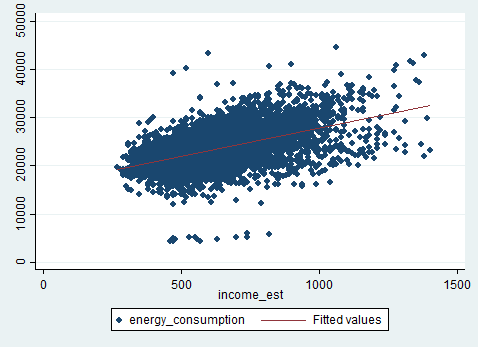
\includegraphics[width=8cm]{../stata_code/ols.png}
    \centering
    \end{figure}
\end{frame}
  
\begin{frame}[fragile]
    \frametitle{Applying Panel Data Methods to Other Data Structures}
    \framesubtitle{Fixed Effects}
    When we use a fixed effects model to estimate the effect of income on household energy consumption \textit{within} local authorities, the size of the effect changes.
    \tiny
    \begin{CVerbatim}[fontsize=\tiny]
. xtreg energy_consumption income_est, fe

Fixed-effects (within) regression               Number of obs     =      7,133
Group variable: LA_CODE                         Number of groups  =        376

R-sq:                                           Obs per group:
     within  = 0.5160                                         min =          1
     between = 0.1057                                         avg =       19.0
     overall = 0.2795                                         max =        131

                                                F(1,6756)         =    7201.69
corr(u_i, Xb)  = -0.5247                        Prob > F          =     0.0000

------------------------------------------------------------------------------
energy_con~n |      Coef.   Std. Err.      t    P>|t|     [95% Conf. Interval]
-------------+----------------------------------------------------------------
  income_est |   20.11081   .2369803    84.86   0.000     19.64625    20.57536
       _cons |   11040.14   145.7513    75.75   0.000     10754.42    11325.86
-------------+----------------------------------------------------------------
     sigma_u |  2773.6255
     sigma_e |  2192.6781
         rho |  .61539872   (fraction of variance due to u_i)
------------------------------------------------------------------------------
F test that all u_i=0: F(375, 6756) = 20.47                  Prob > F = 0.0000
    
    \end{CVerbatim}
    
{
\begin{table}[htbp]\centering
 \caption{Estimation results : xtreg
\label{tabresult xtreg}}
\begin{tabular}{l c c }\hline\hline 
\multicolumn{1}{c}
{\textbf{Variable}}
 & {\textbf{Coefficient}}  & \textbf{(Std. Err.)} \\ \hline
income\_est  &  20.111  & (0.237)\\
Intercept  &  11040.143  & (145.751)\\
\hline\end{tabular}
\end{table}
}


\end{frame}
  
\begin{frame}[fragile]
    \frametitle{Applying Panel Data Methods to Other Data Structures}
    \framesubtitle{Fixed Effects}
    \tiny
    \begin{CVerbatim}[fontsize=\tiny]
. xi: regress energy_consumption income_est i.LA_CODE
. predict energy_consumption_fitted
(option xb assumed; fitted values)
. separate energy_consumption, by(LA_CODE)
. separate energy_consumption_fitted, by(LA_CODE)
. graph twoway (scatter energy_consumption1-energy_consumption80 income_est) ///
>         (line energy_consumption_fitted1-energy_consumption_fitted80 income_est) ///
>         (lfit energy_consumption income_est, ///
>         color(black) lwidth(thick) lpattern(dash)), legend(off) 
    \end{CVerbatim}
    
    \begin{figure}
    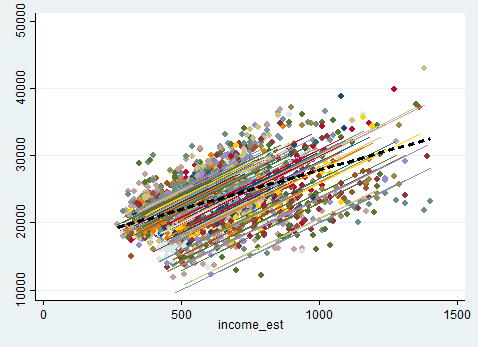
\includegraphics[width=7cm]{../stata_code/fe.png}
    \centering
    \end{figure}
\end{frame}
  
\begin{frame}[fragile]
    \frametitle{Applying Panel Data Methods to Other Data Structures}
    \framesubtitle{Comparing OLS with Fixed Effects Models}
    \tiny
    \begin{CVerbatim}[fontsize=\tiny]
. esttab ols fe

--------------------------------------------
                      (1)             (2)   
             energy_con~n    energy_con~n   
--------------------------------------------
income_est          11.68***        20.11***
                  (52.60)         (84.86)   

_cons             16142.1***      11040.1***
                 (115.81)         (75.75)   
--------------------------------------------
N                    7133            7133   
--------------------------------------------
t statistics in parentheses
* p<0.05, ** p<0.01, *** p<0.001
    \end{CVerbatim}

\end{frame}

\end{document}